\section*{Question 2}

We solve and simulate two model variants: the baseline with $\tau = 0.3$ and a counterfactual with no labor income tax ($\tau = 0$). Note that the cohort wage constants are corrected to $(\alpha_0,\alpha_1,\alpha_2,\alpha_3,\alpha_4) = (0.7, 0.8, 0.9, 1.1, 1.2)$ as specified, replacing the linear interpolation in the starter code.
\begin{figure}[H]
  \centering
  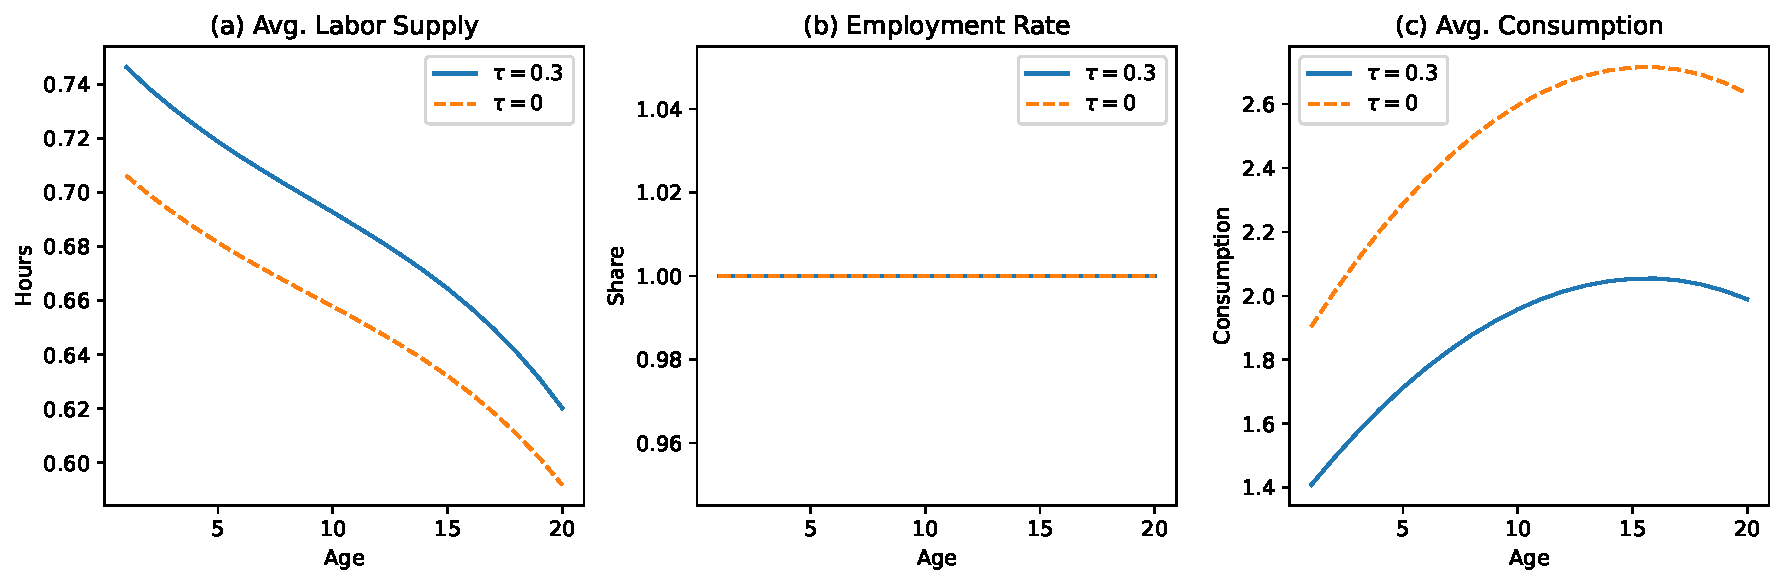
\includegraphics[width=\textwidth]{../figures/q2_age_profiles.pdf}
  \caption{Age profiles for $\tau = 0.3$ (baseline) and $\tau = 0$ (no-tax counterfactual).}
  \label{fig:q2}
\end{figure}
The tax \emph{raises} labor supply throughout the life cycle: the $\tau = 0.3$ profile lies above $\tau = 0$ at every age (Figure~\ref{fig:q2}a). With $\rho = 1.5 > 1$ the income effect dominates the substitution effect, so a lower net wage induces workers to supply more hours to defend their consumption. The employment rate is $100\%$ in both economies: $\pi_0 = 0.5$ is never attractive enough to pull anyone out of work at these tax rates, as the Laffer analysis in Question~3 confirms. Consumption is nonetheless higher under $\tau = 0$ at every age, since workers retain their full earnings, and the $(1-\tau)$ wedge outweighs the modestly higher hours and human capital that the tax induces.